\chapter{Geometria}

\index{geometry}

Em problemas geométricos, geralmente é desafiador encontrar uma maneira de abordar o problema de forma que a solução possa ser implementada convenientemente e o número de casos especiais seja pequeno.

Como exemplo, considere um problema em que são dados os vértices de um quadrilátero (um polígono que possui quatro vértices) e nossa tarefa é calcular sua área. Por exemplo, uma entrada possível para o problema é a seguinte:

\begin{center}
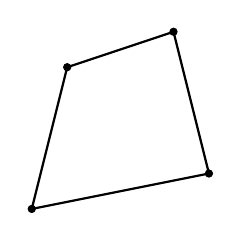
\begin{tikzpicture}[scale=0.45]

\draw[fill] (6,2) circle [radius=0.1];
\draw[fill] (5,6) circle [radius=0.1];
\draw[fill] (2,5) circle [radius=0.1];
\draw[fill] (1,1) circle [radius=0.1];
\draw[thick] (6,2) -- (5,6) -- (2,5) -- (1,1) -- (6,2);
\end{tikzpicture}
\end{center}
Uma maneira de abordar o problema é dividir o quadrilátero em dois triângulos por uma linha reta entre dois vértices opostos:
\begin{center}
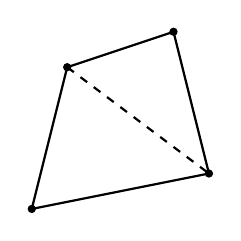
\begin{tikzpicture}[scale=0.45]

\draw[fill] (6,2) circle [radius=0.1];
\draw[fill] (5,6) circle [radius=0.1];
\draw[fill] (2,5) circle [radius=0.1];
\draw[fill] (1,1) circle [radius=0.1];

\draw[thick] (6,2) -- (5,6) -- (2,5) -- (1,1) -- (6,2);
\draw[dashed,thick] (2,5) -- (6,2);
\end{tikzpicture}
\end{center}
Após isso, basta somar as áreas dos triângulos. A área de um triângulo pode ser calculada, por exemplo, usando a \key{fórmula de Heron}
%\footnote{Heron of Alexandria (c. 10--70) was a Greek mathematician.}
\[ \sqrt{s (s-a) (s-b) (s-c)},\]
onde $a$, $b$ e $c$ são os comprimentos dos lados do triângulo e
$s=(a+b+c)/2$.
\index{Heron's formula}

Esta é uma maneira possível de resolver o problema, mas há uma armadilha: como dividir o quadrilátero em triângulos? Acontece que às vezes não podemos simplesmente escolher dois vértices opostos arbitrários. Por exemplo, na seguinte situação, a linha de divisão está \emph{fora} do quadrilátero:
\begin{center}
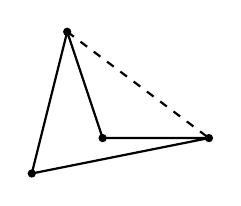
\begin{tikzpicture}[scale=0.45]

\draw[fill] (6,2) circle [radius=0.1];
\draw[fill] (3,2) circle [radius=0.1];
\draw[fill] (2,5) circle [radius=0.1];
\draw[fill] (1,1) circle [radius=0.1];
\draw[thick] (6,2) -- (3,2) -- (2,5) -- (1,1) -- (6,2);

\draw[dashed,thick] (2,5) -- (6,2);
\end{tikzpicture}
\end{center}
No entanto, outra maneira de desenhar a linha funciona:
\begin{center}
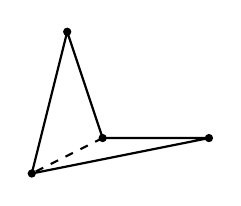
\begin{tikzpicture}[scale=0.45]

\draw[fill] (6,2) circle [radius=0.1];
\draw[fill] (3,2) circle [radius=0.1];
\draw[fill] (2,5) circle [radius=0.1];
\draw[fill] (1,1) circle [radius=0.1];
\draw[thick] (6,2) -- (3,2) -- (2,5) -- (1,1) -- (6,2);

\draw[dashed,thick] (3,2) -- (1,1);
\end{tikzpicture}
\end{center}
É claro para um humano qual das linhas é a escolha correta, mas a situação é difícil para um computador.

No entanto, verifica-se que podemos resolver o problema usando outro método que é mais conveniente para um programador. Ou seja, existe uma fórmula geral
\[x_1y_2-x_2y_1+x_2y_3-x_3y_2+x_3y_4-x_4y_3+x_4y_1-x_1y_4,\]
que calcula a área de um quadrilátero cujos vértices são
$(x_1,y_1)$,
$(x_2,y_2)$,
$(x_3,y_3)$ e
$(x_4,y_4)$.
Esta fórmula é fácil de implementar, não há casos especiais e podemos até generalizar a fórmula para \emph{todos} os polígonos.

\section{Números Complexos}

\index{complex number}
\index{point}
\index{vector}

Um \key{número complexo} é um número da forma $x+y i$,
onde $i = \sqrt{-1}$ é a \key{unidade imaginária}.
Uma interpretação geométrica de um número complexo é
que ele representa um ponto bidimensional $(x,y)$
ou um vetor da origem para um ponto $(x,y)$.

Por exemplo, $4+2i$ corresponde ao
seguinte ponto e vetor:

\begin{center}
\begin{tikzpicture}[scale=0.45]

\draw[->,thick] (-5,0)--(5,0);
\draw[->,thick] (0,-5)--(0,5);

\draw[fill] (4,2) circle [radius=0.1];
\draw[->,thick] (0,0)--(4-0.1,2-0.1);

\node at (4,2.8) {$(4,2)$};
\end{tikzpicture}
\end{center}

\index{complex@\texttt{complex}}

A classe de número complexo \texttt{complex} do C++ é
útil ao resolver problemas geométricos.
Usando a classe, podemos representar pontos e vetores
como números complexos, e a classe contém ferramentas
que são úteis em geometria.

No código a seguir, \texttt{C} é o tipo de
uma coordenada e \texttt{P} é o tipo de um ponto ou um vetor.
Além disso, o código define as macros \texttt{X} e \texttt{Y}
que podem ser usadas para se referir às coordenadas x e y.

\begin{lstlisting}
typedef long long C;
typedef complex<C> P;
#define X real()
#define Y imag()
\end{lstlisting}

Por exemplo, o código a seguir define um ponto $p=(4,2)$
e imprime suas coordenadas x e y:

\begin{lstlisting}
P p = {4,2};
cout << p.X << " " << p.Y << "\n"; // 4 2
\end{lstlisting}

O código a seguir define os vetores $v=(3,1)$ e $u=(2,2)$,
e depois calcula a soma $s=v+u$.

\begin{lstlisting}
P v = {3,1};
P u = {2,2};
P s = v+u;
cout << s.X << " " << s.Y << "\n"; // 5 3
\end{lstlisting}

Na prática,
um tipo de coordenada apropriado é geralmente
\texttt{long long} (inteiro) ou \texttt{long double}
(número real).
É uma boa ideia usar inteiro sempre que possível,
porque os cálculos com inteiros são exatos.
Se números reais forem necessários,
os erros de precisão devem ser levados em consideração
ao comparar números.
Uma maneira segura de verificar se os números reais $a$ e $b$ são iguais
é compará-los usando $|a-b|<\epsilon$,
onde $\epsilon$ é um número pequeno (por exemplo, $\epsilon=10^{-9}$).

\subsubsection*{Funções}

Nos exemplos a seguir, o tipo de coordenada é
\texttt{long double}.

A função $\texttt{abs}(v)$ calcula o comprimento
$|v|$ de um vetor $v=(x,y)$
usando a fórmula $\sqrt{x^2+y^2}$.
A função também pode ser usada para
calcular a distância entre os pontos
$(x_1,y_1)$ e $(x_2,y_2)$,
porque essa distância é igual ao comprimento
do vetor $(x_2-x_1,y_2-y_1)$.

O código a seguir calcula a distância
entre os pontos $(4,2)$ e $(3,-1)$:
\begin{lstlisting}
P a = {4,2};
P b = {3,-1};
cout << abs(b-a) << "\n"; // 3.16228
\end{lstlisting}

A função $\texttt{arg}(v)$ calcula o
ângulo de um vetor $v=(x,y)$ em relação ao eixo x.
A função fornece o ângulo em radianos,
onde $r$ radianos é igual a $180 r/\pi$ graus.
O ângulo de um vetor que aponta para a direita é 0,
e os ângulos diminuem no sentido horário e aumentam
no sentido anti-horário.

A função $\texttt{polar}(s,a)$ constrói um vetor
cujo comprimento é $s$ e que aponta para um ângulo $a$.
Um vetor pode ser girado por um ângulo $a$
multiplicando-o por um vetor com comprimento 1 e ângulo $a$.

O código a seguir calcula o ângulo de
o vetor $(4,2)$, gira-o $1/2$ radianos
no sentido anti-horário e, em seguida, calcula o ângulo novamente:

\begin{lstlisting}
P v = {4,2};
cout << arg(v) << "\n"; // 0.463648
v *= polar(1.0,0.5);
cout << arg(v) << "\n"; // 0.963648
\end{lstlisting}

\section{Pontos e Linhas}

\index{cross product}

O \key{produto vetorial} $a \times b$ de vetores
$a=(x_1,y_1)$ e $b=(x_2,y_2)$ é calculado
usando a fórmula $x_1 y_2 - x_2 y_1$.
O produto vetorial nos diz se $b$
gira para a esquerda (valor positivo), não gira (zero)
ou gira para a direita (valor negativo)
quando é colocado diretamente após $a$.

A figura a seguir ilustra os casos acima:
\begin{center}
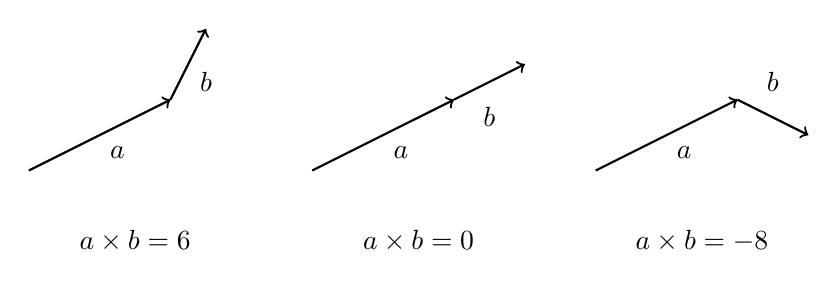
\begin{tikzpicture}[scale=0.45]

\draw[->,thick] (0,0)--(4,2);
\draw[->,thick] (4,2)--(4+1,2+2);

\node at (2.5,0.5) {$a$};
\node at (5,2.5) {$b$};

\node at (3,-2) {$a \times b = 6$};

\draw[->,thick] (8+0,0)--(8+4,2);
\draw[->,thick] (8+4,2)--(8+4+2,2+1);

\node at (8+2.5,0.5) {$a$};
\node at (8+5,1.5) {$b$};

\node at (8+3,-2) {$a \times b = 0$};

\draw[->,thick] (16+0,0)--(16+4,2);
\draw[->,thick] (16+4,2)--(16+4+2,2-1);

\node at (16+2.5,0.5) {$a$};
\node at (16+5,2.5) {$b$};

\node at (16+3,-2) {$a \times b = -8$};
\end{tikzpicture}
\end{center}

\noindent
Por exemplo, no primeiro caso
$a=(4,2)$ e $b=(1,2)$.
O código a seguir calcula o produto vetorial
usando a classe \texttt{complex}:

\begin{lstlisting}
P a = {4,2};
P b = {1,2};
C p = (conj(a)*b).Y; // 6
\end{lstlisting}

O código acima funciona porque
a função \texttt{conj} inverte o sinal da coordenada y
de um vetor,
e quando os vetores $(x_1,-y_1)$ e $(x_2,y_2)$
são multiplicados, a coordenada y
do resultado é $x_1 y_2 - x_2 y_1$.

\subsubsection{Localização do Ponto}

Produtos vetoriais podem ser usados para testar
se um ponto está localizado à esquerda ou à direita
de uma linha.
Assuma que a linha passa pelos pontos
$s_1$ e $s_2$, estamos olhando de $s_1$
para $s_2$ e o ponto é $p$.

Por exemplo, na figura a seguir,
$p$ está no lado esquerdo da linha:
\begin{center}
\begin{tikzpicture}[scale=0.45]
\draw[dashed,thick,->] (0,-3)--(12,6);
\draw[fill] (4,0) circle [radius=0.1];
\draw[fill] (8,3) circle [radius=0.1];
\draw[fill] (5,3) circle [radius=0.1];
\node at (4,-1) {$s_1$};
\node at (8,2) {$s_2$};
\node at (5,4) {$p$};
\end{tikzpicture}
\end{center}

O produto vetorial $(p-s_1) \times (p-s_2)$
nos diz a localização do ponto $p$.
Se o produto vetorial for positivo,
$p$ está localizado no lado esquerdo,
e se o produto vetorial for negativo,
$p$ está localizado no lado direito.
Finalmente, se o produto vetorial for zero,
os pontos $s_1$, $s_2$ e $p$ estão na mesma linha.

\subsubsection{Interseção de Segmentos de Linha}

\index{line segment intersection}

A seguir, consideramos o problema de testar
se dois segmentos de linha
$ab$ e $cd$ se cruzam. Os casos possíveis são:

\textit{Caso 1:}
Os segmentos de linha estão na mesma linha
e eles se sobrepõem.
Nesse caso, há um número infinito de
pontos de interseção.
Por exemplo, na figura a seguir,
todos os pontos entre $c$ e $b$ são
pontos de interseção:
\begin{center}
\begin{tikzpicture}[scale=0.9]
\draw (1.5,1.5)--(6,3);
\draw (0,1)--(4.5,2.5);
\draw[fill] (0,1) circle [radius=0.05];
\node at (0,0.5) {$a$};
\draw[fill] (1.5,1.5) circle [radius=0.05];
\node at (6,2.5) {$d$};
\draw[fill] (4.5,2.5) circle [radius=0.05];
\node at (1.5,1) {$c$};
\draw[fill] (6,3) circle [radius=0.05];
\node at (4.5,2) {$b$};
\end{tikzpicture}
\end{center}

Neste caso, podemos usar produtos vetoriais para
verificar se todos os pontos estão na mesma linha.
Depois disso, podemos classificar os pontos e verificar
se os segmentos de linha se sobrepõem.

\textit{Caso 2:}
Os segmentos de linha têm um vértice comum
que é o único ponto de interseção.
Por exemplo, na figura a seguir o
ponto de interseção é $b=c$:

\begin{center}
\begin{tikzpicture}[scale=0.9]
\draw (0,0)--(4,2);
\draw (4,2)--(6,1);
\draw[fill] (0,0) circle [radius=0.05];
\draw[fill] (4,2) circle [radius=0.05];
\draw[fill] (6,1) circle [radius=0.05];

\node at (0,0.5) {$a$};
\node at (4,2.5) {$b=c$};
\node at (6,1.5) {$d$};
\end{tikzpicture}
\end{center}

Este caso é fácil de verificar, porque
existem apenas quatro possibilidades
para o ponto de interseção:
$a=c$, $a=d$, $b=c$ e $b=d$.

\textit{Caso 3:}
Existe exatamente um ponto de interseção
que não é um vértice de nenhum segmento de linha.
Na figura a seguir, o ponto $p$
é o ponto de interseção:
\begin{center}
\begin{tikzpicture}[scale=0.9]
\draw (0,1)--(6,3);
\draw (2,4)--(4,0);
\draw[fill] (0,1) circle [radius=0.05];
\node at (0,0.5) {$c$};
\draw[fill] (6,3) circle [radius=0.05];
\node at (6,2.5) {$d$};
\draw[fill] (2,4) circle [radius=0.05];
\node at (1.5,3.5) {$a$};
\draw[fill] (4,0) circle [radius=0.05];
\node at (4,-0.4) {$b$};
\draw[fill] (3,2) circle [radius=0.05];
\node at (3,1.5) {$p$};
\end{tikzpicture}
\end{center}

Neste caso, os segmentos de linha se cruzam
exatamente quando ambos os pontos $c$ e $d$ estão
em lados diferentes de uma linha que passa por $a$ e $b$,
e os pontos $a$ e $b$ estão em diferentes
lados de uma linha que passa por $c$ e $d$.
Podemos usar produtos vetoriais para verificar isso.

\subsubsection{Distância de um Ponto a uma Linha}

Outra característica dos produtos vetoriais é que
a área de um triângulo pode ser calculada
usando a fórmula
\[\frac{| (a-c) \times (b-c) |}{2},\]
onde $a$, $b$ e $c$ são os vértices do triângulo.
Usando esse fato, podemos derivar uma fórmula
para calcular a distância mais curta entre um ponto e uma linha.
Por exemplo, na figura a seguir $d$ é a
distância mais curta entre o ponto $p$ e a linha
que é definida pelos pontos $s_1$ e $s_2$:
\begin{center}
\begin{tikzpicture}[scale=0.75]
\draw (-2,-1)--(6,3);
\draw[dashed] (1,4)--(2.40,1.2);
\node at (0,-0.5) {$s_1$};
\node at (4,1.5) {$s_2$};
\node at (0.5,4) {$p$};
\node at (2,2.7) {$d$};
\draw[fill] (0,0) circle [radius=0.05];
\draw[fill] (4,2) circle [radius=0.05];
\draw[fill] (1,4) circle [radius=0.05];
\end{tikzpicture}
\end{center}

A área do triângulo cujos vértices são
$s_1$, $s_2$ e $p$ podem ser calculados de duas maneiras:
é ambos
$\frac{1}{2} |s_2-s_1| d$ e
$\frac{1}{2} ((s_1-p) \times (s_2-p))$.
Assim, a distância mais curta é
\[ d = \frac{(s_1-p) \times (s_2-p)}{|s_2-s_1|} .\]

\subsubsection{Ponto Dentro de um Polígono}

Vamos agora considerar o problema de
testar se um ponto está localizado dentro ou fora
de um polígono.
Por exemplo, na figura a seguir, o ponto $a$
está dentro do polígono e o ponto $b$ está fora
do polígono.

\begin{center}
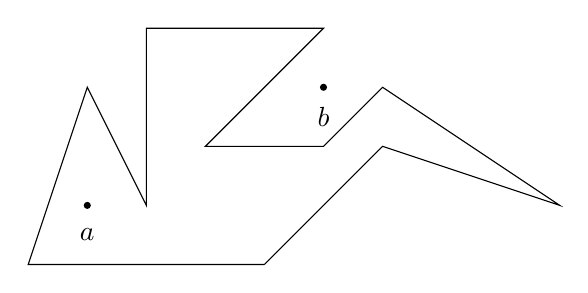
\begin{tikzpicture}[scale=0.75]
%\draw (0,0)--(2,-2)--(3,1)--(5,1)--(2,3)--(1,2)--(-1,2)--(1,4)--(-2,4)--(-2,1)--(-3,3)--(-4,0)--(0,0);
\draw (0,0)--(2,2)--(5,1)--(2,3)--(1,2)--(-1,2)--(1,4)--(-2,4)--(-2,1)--(-3,3)--(-4,0)--(0,0);

\draw[fill] (-3,1) circle [radius=0.05];
\node at (-3,0.5) {$a$};
\draw[fill] (1,3) circle [radius=0.05];
\node at (1,2.5) {$b$};
\end{tikzpicture}
\end{center}

Uma maneira conveniente de resolver o problema é
enviar um \emph{raio} do ponto para uma direção arbitrária
e calcular o número de vezes que ele toca
a fronteira do polígono.
Se o número for ímpar,
o ponto está dentro do polígono,
e se o número for par,
o ponto está fora do polígono.

\begin{samepage}
Por exemplo, podemos enviar os seguintes raios:
\begin{center}
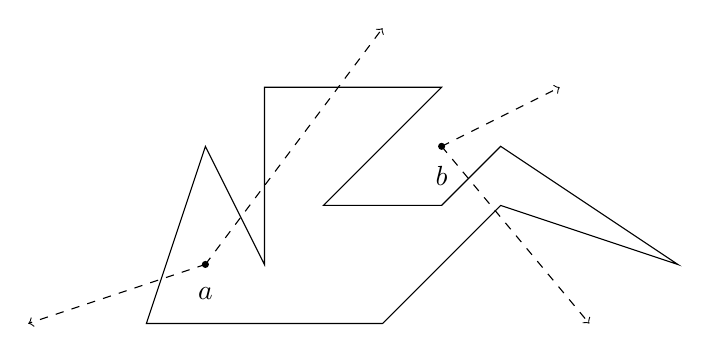
\begin{tikzpicture}[scale=0.75]
\draw (0,0)--(2,2)--(5,1)--(2,3)--(1,2)--(-1,2)--(1,4)--(-2,4)--(-2,1)--(-3,3)--(-4,0)--(0,0);

\draw[fill] (-3,1) circle [radius=0.05];
\node at (-3,0.5) {$a$};
\draw[fill] (1,3) circle [radius=0.05];
\node at (1,2.5) {$b$};

\draw[dashed,->] (-3,1)--(-6,0);
\draw[dashed,->] (-3,1)--(0,5);

\draw[dashed,->] (1,3)--(3.5,0);
\draw[dashed,->] (1,3)--(3,4);
\end{tikzpicture}
\end{center}
\end{samepage}

Os raios de $a$ tocam 1 e 3 vezes
a fronteira do polígono,
então $a$ está dentro do polígono.
Correspondentemente, os raios de $b$
tocam 0 e 2 vezes a fronteira do polígono,
então $b$ está fora do polígono.

\section{Área do Polígono}

Uma fórmula geral para calcular a área
de um polígono, às vezes chamada de \key{fórmula do cadarço},
é como se segue: \index{shoelace formula}
\[\frac{1}{2} |\sum_{i=1}^{n-1} (p_i \times p_{i+1})| =
\frac{1}{2} |\sum_{i=1}^{n-1} (x_i y_{i+1} - x_{i+1} y_i)|, \]
Aqui, os vértices são
$p_1=(x_1,y_1)$, $p_2=(x_2,y_2)$, $\ldots$, $p_n=(x_n,y_n)$
em uma ordem tal que
$p_i$ e $p_{i+1}$ são vértices adjacentes na fronteira
do polígono,
e o primeiro e o último vértice são iguais, ou seja, $p_1=p_n$.

Por exemplo, a área do polígono
\begin{center}
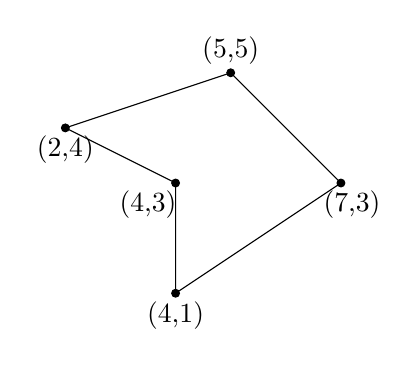
\begin{tikzpicture}[scale=0.7]
\filldraw (4,1.4) circle (2pt);
\filldraw (7,3.4) circle (2pt);
\filldraw (5,5.4) circle (2pt);
\filldraw (2,4.4) circle (2pt);
\filldraw (4,3.4) circle (2pt);
\node (1) at (4,1) {(4,1)};
\node (2) at (7.2,3) {(7,3)};
\node (3) at (5,5.8) {(5,5)};
\node (4) at (2,4) {(2,4)};
\node (5) at (3.5,3) {(4,3)};
\path[draw] (4,1.4) -- (7,3.4) -- (5,5.4) -- (2,4.4) -- (4,3.4) -- (4,1.4);
\end{tikzpicture}
\end{center}
é
\[\frac{|(2\cdot5-5\cdot4)+(5\cdot3-7\cdot5)+(7\cdot1-4\cdot3)+(4\cdot3-4\cdot1)+(4\cdot4-2\cdot3)|}{2} = 17/2.\]

A ideia da fórmula é passar por trapézios
cujo um lado é um lado do polígono,
e o outro lado fica na linha horizontal $y=0$.
Por exemplo:
\begin{center}
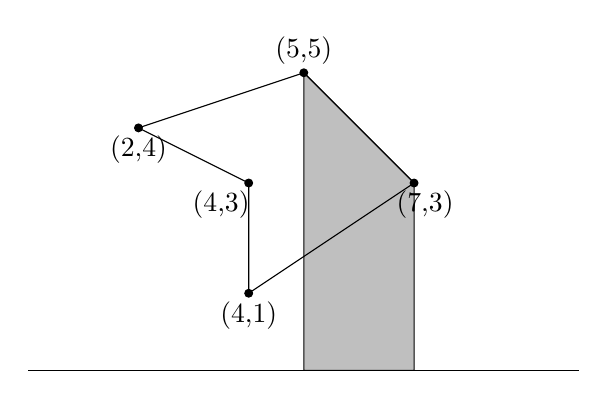
\begin{tikzpicture}[scale=0.7]
\path[draw,fill=lightgray] (5,5.4) -- (7,3.4) -- (7,0) -- (5,0) -- (5,5.4);
\filldraw (4,1.4) circle (2pt);
\filldraw (7,3.4) circle (2pt);
\filldraw (5,5.4) circle (2pt);
\filldraw (2,4.4) circle (2pt);
\filldraw (4,3.4) circle (2pt);
\node (1) at (4,1) {(4,1)};
\node (2) at (7.2,3) {(7,3)};
\node (3) at (5,5.8) {(5,5)};
\node (4) at (2,4) {(2,4)};
\node (5) at (3.5,3) {(4,3)};
\path[draw] (4,1.4) -- (7,3.4) -- (5,5.4) -- (2,4.4) -- (4,3.4) -- (4,1.4);
\draw (0,0) -- (10,0);
\end{tikzpicture}
\end{center}
A área de tal trapézio é
\[(x_{i+1}-x_{i}) \frac{y_i+y_{i+1}}{2},\]
onde os vértices do polígono são $p_i$ e $p_{i+1}$.
Se $x_{i+1}>x_{i}$, a área é positiva,
e se $x_{i+1}<x_{i}$, a área é negativa.

A área do polígono é a soma das áreas de
todos esses trapézios, o que produz a fórmula
\[|\sum_{i=1}^{n-1} (x_{i+1}-x_{i}) \frac{y_i+y_{i+1}}{2}| =
\frac{1}{2} |\sum_{i=1}^{n-1} (x_i y_{i+1} - x_{i+1} y_i)|.\]

Observe que o valor absoluto da soma é considerado,
porque o valor da soma pode ser positivo ou negativo,
dependendo se caminhamos no sentido horário ou anti-horário
ao longo da fronteira do polígono.

\subsubsection{Teorema de Pick}

\index{Pick's theorem}

O \key{Teorema de Pick} fornece outra maneira de calcular
a área de um polígono, desde que todos os vértices
do polígono tenham coordenadas inteiras.
De acordo com o Teorema de Pick, a área do polígono é
\[ a + b/2 -1,\]
onde $a$ é o número de pontos inteiros dentro do polígono
e $b$ é o número de pontos inteiros na fronteira do polígono.

Por exemplo, a área do polígono
\begin{center}
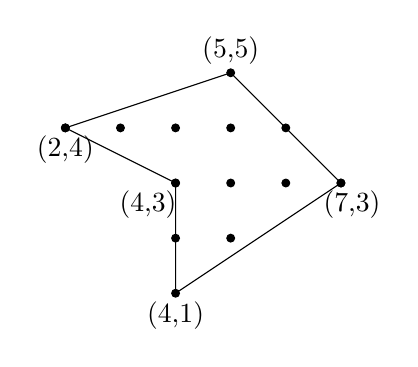
\begin{tikzpicture}[scale=0.7]
\filldraw (4,1.4) circle (2pt);
\filldraw (7,3.4) circle (2pt);
\filldraw (5,5.4) circle (2pt);
\filldraw (2,4.4) circle (2pt);
\filldraw (4,3.4) circle (2pt);
\node (1) at (4,1) {(4,1)};
\node (2) at (7.2,3) {(7,3)};
\node (3) at (5,5.8) {(5,5)};
\node (4) at (2,4) {(2,4)};
\node (5) at (3.5,3) {(4,3)};
\path[draw] (4,1.4) -- (7,3.4) -- (5,5.4) -- (2,4.4) -- (4,3.4) -- (4,1.4);

\filldraw (2,4.4) circle (2pt);
\filldraw (3,4.4) circle (2pt);
\filldraw (4,4.4) circle (2pt);
\filldraw (5,4.4) circle (2pt);
\filldraw (6,4.4) circle (2pt);

\filldraw (4,3.4) circle (2pt);
\filldraw (5,3.4) circle (2pt);
\filldraw (6,3.4) circle (2pt);
\filldraw (7,3.4) circle (2pt);

\filldraw (4,2.4) circle (2pt);
\filldraw (5,2.4) circle (2pt);
\end{tikzpicture}
\end{center}
é $6+7/2-1=17/2$.

\section{Funções de Distância}

\index{distance function}
\index{Euclidean distance}
\index{Manhattan distance}

Uma \key{função de distância} define a distância entre
dois pontos.
A função de distância usual é a
\key{distância euclidiana} onde a distância entre
os pontos $(x_1,y_1)$ e $(x_2,y_2)$ é
\[\sqrt{(x_2-x_1)^2+(y_2-y_1)^2}.\]
Uma função de distância alternativa é a
\key{distância de Manhattan},
onde a distância entre os pontos
$(x_1,y_1)$ e $(x_2,y_2)$ é
\[|x_1-x_2|+|y_1-y_2|.\]
\begin{samepage}
Por exemplo, considere a seguinte imagem:
\begin{center}
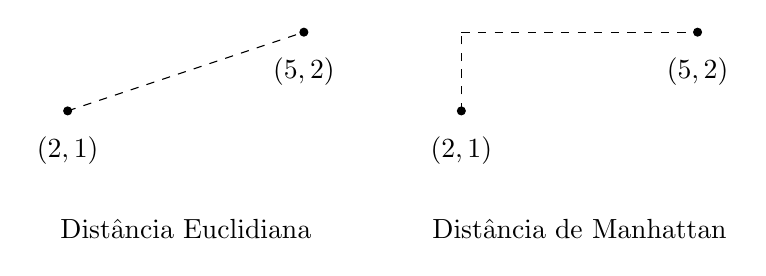
\begin{tikzpicture}

\draw[fill] (2,1) circle [radius=0.05];
\draw[fill] (5,2) circle [radius=0.05];

\node at (2,0.5) {$(2,1)$};
\node at (5,1.5) {$(5,2)$};

\draw[dashed] (2,1) -- (5,2);

\draw[fill] (5+2,1) circle [radius=0.05];
\draw[fill] (5+5,2) circle [radius=0.05];

\node at (5+2,0.5) {$(2,1)$};
\node at (5+5,1.5) {$(5,2)$};

\draw[dashed] (5+2,1) -- (5+2,2);
\draw[dashed] (5+2,2) -- (5+5,2);

\node at (3.5,-0.5) {Distância Euclidiana};
\node at (5+3.5,-0.5) {Distância de Manhattan};
\end{tikzpicture}
\end{center}
\end{samepage}
A distância euclidiana entre os pontos é
\[\sqrt{(5-2)^2+(2-1)^2}=\sqrt{10}\]
e a distância de Manhattan é
\[|5-2|+|2-1|=4.\]
A figura a seguir mostra as regiões que estão a uma distância de 1
do ponto central, usando as distâncias euclidiana e de Manhattan:
\begin{center}
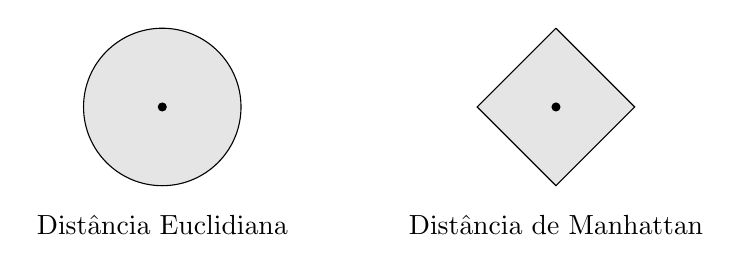
\begin{tikzpicture}

\draw[fill=gray!20] (0,0) circle [radius=1];
\draw[fill] (0,0) circle [radius=0.05];

\node at (0,-1.5) {Distância Euclidiana};

\draw[fill=gray!20] (5+0,1) -- (5-1,0) -- (5+0,-1) -- (5+1,0) -- (5+0,1);
\draw[fill] (5,0) circle [radius=0.05];
\node at (5,-1.5) {Distância de Manhattan};
\end{tikzpicture}
\end{center}

\subsubsection{Rotação de Coordenadas}

Alguns problemas são mais fáceis de resolver se
as distâncias de Manhattan forem usadas em vez das distâncias euclidianas.
Como exemplo, considere um problema em que recebemos
$n$ pontos no plano bidimensional
e nossa tarefa é calcular a distância máxima de Manhattan
entre quaisquer dois pontos.

Por exemplo, considere o seguinte conjunto de pontos:
\begin{center}
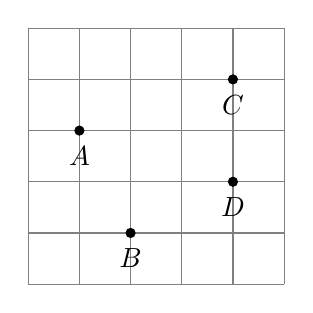
\begin{tikzpicture}[scale=0.65]
\draw[color=gray] (-1,-1) grid (4,4);

\filldraw (0,2) circle (2.5pt);
\filldraw (3,3) circle (2.5pt);
\filldraw (1,0) circle (2.5pt);
\filldraw (3,1) circle (2.5pt);

\node at (0,1.5) {$A$};
\node at (3,2.5) {$C$};
\node at (1,-0.5) {$B$};
\node at (3,0.5) {$D$};
\end{tikzpicture}
\end{center}
A distância máxima de Manhattan é 5
entre os pontos $B$ e $C$:
\begin{center}
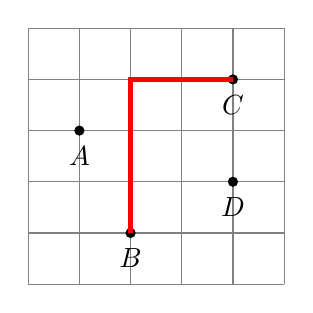
\begin{tikzpicture}[scale=0.65]
\draw[color=gray] (-1,-1) grid (4,4);

\filldraw (0,2) circle (2.5pt);
\filldraw (3,3) circle (2.5pt);
\filldraw (1,0) circle (2.5pt);
\filldraw (3,1) circle (2.5pt);

\node at (0,1.5) {$A$};
\node at (3,2.5) {$C$};
\node at (1,-0.5) {$B$};
\node at (3,0.5) {$D$};

\path[draw=red,thick,line width=2pt] (1,0) -- (1,3) -- (3,3);
\end{tikzpicture}
\end{center}

Uma técnica útil relacionada às distâncias de Manhattan
é girar todas as coordenadas 45 graus para que
um ponto $(x,y)$ se torne $(x+y,y-x)$.
Por exemplo, após girar os pontos acima,
o resultado é:

\begin{center}
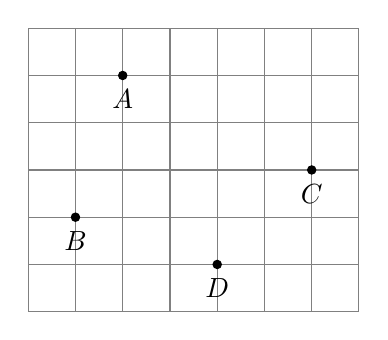
\begin{tikzpicture}[scale=0.6]
\draw[color=gray] (0,-3) grid (7,3);

\filldraw (2,2) circle (2.5pt);
\filldraw (6,0) circle (2.5pt);
\filldraw (1,-1) circle (2.5pt);
\filldraw (4,-2) circle (2.5pt);

\node at (2,1.5) {$A$};
\node at (6,-0.5) {$C$};
\node at (1,-1.5) {$B$};
\node at (4,-2.5) {$D$};
\end{tikzpicture}
\end{center}
E a distância máxima é a seguinte:
\begin{center}
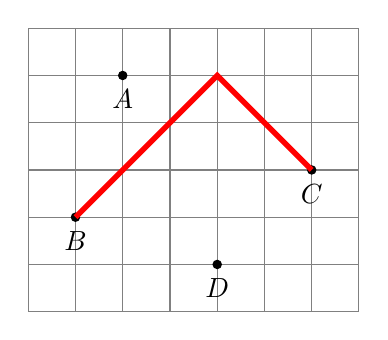
\begin{tikzpicture}[scale=0.6]
\draw[color=gray] (0,-3) grid (7,3);

\filldraw (2,2) circle (2.5pt);
\filldraw (6,0) circle (2.5pt);
\filldraw (1,-1) circle (2.5pt);
\filldraw (4,-2) circle (2.5pt);

\node at (2,1.5) {$A$};
\node at (6,-0.5) {$C$};
\node at (1,-1.5) {$B$};
\node at (4,-2.5) {$D$};

\path[draw=red,thick,line width=2pt] (1,-1) -- (4,2) -- (6,0);
\end{tikzpicture}
\end{center}

Considere dois pontos $p_1=(x_1,y_1)$ e $p_2=(x_2,y_2)$ cujas coordenadas
giradas são $p'_1=(x'_1,y'_1)$ e $p'_2=(x'_2,y'_2)$.
Agora, existem duas maneiras de expressar a distância de Manhattan
entre $p_1$ e $p_2$:
\[|x_1-x_2|+|y_1-y_2| = \max(|x'_1-x'_2|,|y'_1-y'_2|)\]

Por exemplo, se $p_1=(1,0)$ e $p_2=(3,3)$,
as coordenadas giradas são $p'_1=(1,-1)$ e $p'_2=(6,0)$
e a distância de Manhattan é
\[|1-3|+|0-3| = \max(|1-6|,|-1-0|) = 5.\]

As coordenadas giradas fornecem uma maneira simples
de operar com distâncias de Manhattan, porque podemos
considerar as coordenadas x e y separadamente.
Para maximizar a distância de Manhattan entre dois pontos,
devemos encontrar dois pontos cujas
coordenadas giradas maximizem o valor de
\[\max(|x'_1-x'_2|,|y'_1-y'_2|).\]
Isso é fácil, porque a diferença horizontal ou vertical
das coordenadas giradas deve ser máxima.
